\documentclass[aspectratio=169,11pt]{beamer}
\usetheme{default}
\setbeamertemplate{navigation symbols}{}
\setbeamertemplate{footline}{%
  \hfill\insertframenumber/\inserttotalframenumber\hspace*{4pt}\vspace{2pt}%
}
\usepackage{lmodern}
\usepackage[most]{tcolorbox}
\usepackage{listings}
\usepackage{tikz}
\usetikzlibrary{arrows.meta,positioning,shapes.geometric,fit,backgrounds}
\usepackage{booktabs}
\usepackage{hyperref}

\definecolor{lcgreen}{HTML}{2E7D32}
\definecolor{lcblue}{HTML}{1565C0}
\definecolor{lcorange}{HTML}{EF6C00}
\definecolor{lcred}{HTML}{C62828}
\definecolor{codebg}{HTML}{F5F5F5}
\definecolor{docgray}{gray}{0.55}

\newtcolorbox{conceptbox}[1][]{colback=yellow!20,colframe=yellow!60!black,title=#1,fonttitle=\bfseries,top=2pt,bottom=2pt,left=4pt,right=4pt}
\newtcolorbox{warningbox}[1][]{colback=red!15,colframe=red!60!black,title=#1,fonttitle=\bfseries,top=2pt,bottom=2pt,left=4pt,right=4pt}
\newtcolorbox{tipbox}[1][]{colback=green!10,colframe=green!50!black,title=#1,fonttitle=\bfseries,top=2pt,bottom=2pt,left=4pt,right=4pt}
\newtcolorbox{codebox}[1][]{colback=blue!10,colframe=blue!40!black,title=#1,fonttitle=\bfseries,top=2pt,bottom=2pt,left=4pt,right=4pt}

\lstset{
  basicstyle=\ttfamily\scriptsize,
  backgroundcolor=\color{codebg},
  breaklines=true,
  frame=single,
  rulecolor=\color{blue!40!black},
  keywordstyle=\color{lcblue}\bfseries,
  stringstyle=\color{lcgreen},
  commentstyle=\color{docgray}\itshape,
  language=Python,
  showstringspaces=false,
  tabsize=2,
  xleftmargin=2pt,
  xrightmargin=2pt,
  aboveskip=2pt,
  belowskip=2pt,
}

\newcommand{\docref}[1]{{\scriptsize\color{docgray}[Docs: #1]}}

\title{Production \& LangGraph Platform}
\subtitle{Section 14: Deploying Agents to Production}
\author{LangGraph v1.0.x}
\date{March 2026}

\begin{document}

\frame{\titlepage}

\begin{frame}{Mental Model: Dev to Production}
\setlength{\itemsep}{1pt}
\begin{itemize}
\item \textbf{Development:} Laptop, SQLite, fast iteration, minimal observability
\item \textbf{Staging:} Full stack, PostgreSQL, load testing, monitoring setup
\item \textbf{Production:} Managed infrastructure, high availability, security, compliance
\item LangGraph Platform abstracts away DevOps complexity
\item Deploy once, scale automatically, monitor centrally
\end{itemize}
\vspace{0.15cm}
\begin{conceptbox}[Shift of Focus]
From writing code to operating systems. Reliability, cost, compliance become critical.
\end{conceptbox}
\end{frame}

\begin{frame}{LangGraph Platform Overview}
\setlength{\itemsep}{1pt}
\begin{itemize}
\item \textbf{Cloud-based platform} for LangGraph application deployment
\item Managed execution, persistence, streaming, monitoring
\item Two deployment modes: Cloud (managed) and Self-Hosted
\item API-first: graphs exposed as REST endpoints
\item Built-in support for assistants, cron jobs, human-in-the-loop
\end{itemize}
\vspace{0.15cm}
\begin{tipbox}[What You Don't Manage]
Database scaling, backups, load balancing, SSL, monitoring infrastructure, autoscaling.
\end{tipbox}
\end{frame}

\begin{frame}{LangGraph Cloud: Managed Deployment}
\setlength{\itemsep}{1pt}
\begin{itemize}
\item Anthropic-hosted infrastructure (AWS, GCP, etc.)
\item Automatic scaling, high availability, multi-region
\item Billing per invocation + token usage
\item Integrated with LangSmith for monitoring
\item Zero DevOps required
\end{itemize}
\vspace{0.15cm}
\begin{tipbox}[Best For]
Startups, teams without DevOps, rapid scaling needs, multi-tenant SaaS.
\end{tipbox}
\end{frame}

\begin{frame}{LangGraph Self-Hosted}
\setlength{\itemsep}{1pt}
\begin{itemize}
\item Run LangGraph infrastructure on your own hardware/cloud account
\item Docker containers, Kubernetes, or VM deployment
\item Full control: compliance, data residency, cost optimization
\item Requires DevOps expertise: networking, scaling, backup strategies
\item Lower per-invocation cost at large scale
\end{itemize}
\vspace{0.15cm}
\begin{warningbox}[Trade-off]
More control, more responsibility. On you to manage uptime, security, scaling.
\end{warningbox}
\end{frame}

\begin{frame}{The LangGraph API Server}
\setlength{\itemsep}{1pt}
\begin{itemize}
\item REST endpoints exposing graph execution
\item \texttt{POST /runs} - invoke graph with input
\item \texttt{GET /runs/\{run\_id\}} - poll execution status
\item \texttt{GET /runs/\{run\_id\}/stream} - stream results
\item \texttt{PATCH /runs/\{run\_id\}/resume} - human-in-the-loop approval
\item Authentication via API key, token, or OAuth
\end{itemize}
\vspace{0.15cm}
\begin{conceptbox}[Language Agnostic]
Any client (Python, JS, Go, curl) can invoke graphs via REST.
\end{conceptbox}
\end{frame}

\begin{frame}{Deploying a Graph: langgraph.json}
\setlength{\itemsep}{1pt}
\begin{itemize}
\item Define graphs: path to module, factory function
\item List dependencies: langgraph, langchain, etc.
\item Specify Python version
\item Provide environment variables and secrets
\item Declarative configuration for platform deployment
\end{itemize}
\vspace{0.1cm}
\begin{tipbox}[Configuration]
langgraph.json tells the platform how to build and run your graphs.
\end{tipbox}
\end{frame}

\begin{frame}{Deploying to LangGraph Cloud}
\setlength{\itemsep}{1pt}
\begin{itemize}
\item Run: \texttt{langgraph deploy --name my-assistant}
\item Platform: compiles graph, installs dependencies
\item Output: REST endpoint, API key for access
\item Immediate: HTTPS-enabled, auto-scaling infrastructure
\end{itemize}
\vspace{0.1cm}
\begin{tipbox}[One Command Deploy]
Zero DevOps. Platform handles infrastructure.
\end{tipbox}
\end{frame}

\begin{frame}{Using the Deployed Graph}
\setlength{\itemsep}{1pt}
\begin{itemize}
\item POST to endpoint with input data
\item Include API key in Authorization header
\item Receive run ID immediately
\item Poll status or stream results via GET
\item HTTP REST API; any language can call
\end{itemize}
\vspace{0.1cm}
\begin{tipbox}[Language Agnostic]
Python, JavaScript, Go, curl-all work with REST endpoints.
\end{tipbox}
\end{frame}

\begin{frame}{Assistants API: Creating Agent Instances}
\setlength{\itemsep}{1pt}
\begin{itemize}
\item Assistants = persistent stateful agent instances
\item Each assistant has own thread, config, tools
\item LangGraph manages assistant lifecycle
\item Create, get, delete, invoke, stream
\item Ideal for per-user or per-conversation agents
\end{itemize}
\vspace{0.15cm}
\begin{tipbox}[Use Case]
A conversational agent per user; LangGraph tracks state across messages.
\end{tipbox}
\end{frame}

\begin{frame}{Assistants API Example}
\setlength{\itemsep}{1pt}
\begin{itemize}
\item Create client: \texttt{LangGraphClient(api\_key=...)}
\item Create assistant: \texttt{client.assistants.create(...)}
\item Invoke: \texttt{assistant.runs.invoke(input, thread\_id)}
\item Stream: \texttt{for update in run.stream()}
\item Per-user/conversation state management
\end{itemize}
\vspace{0.1cm}
\begin{tipbox}[Stateful Agents]
Assistants API manages persistence and conversation history.
\end{tipbox}
\end{frame}

\begin{frame}{Cron Jobs \& Background Tasks}
\setlength{\itemsep}{1pt}
\begin{itemize}
\item Schedule graph execution on intervals (daily, hourly, etc.)
\item Examples: periodic data refresh, cleanup tasks, reporting
\item Triggered by cron expression, not HTTP request
\item Results persisted; can be polled or streamed
\end{itemize}
\vspace{0.15cm}
\begin{tipbox}[Use Case]
Daily report generation, periodic model fine-tuning, cache invalidation.
\end{tipbox}
\end{frame}

\begin{frame}{Cron Job Configuration}
\setlength{\itemsep}{1pt}
\begin{itemize}
\item Add \texttt{"cron": "0 9 * * *"} to graph config (9 AM daily)
\item Platform automatically invokes on schedule
\item Results persisted; can poll or stream
\item Examples: daily reports, model fine-tuning, cache refresh
\end{itemize}
\vspace{0.1cm}
\begin{tipbox}[Scheduled Tasks]
No external cron needed. LangGraph handles scheduling.
\end{tipbox}
\end{frame}

\begin{frame}{Monitoring with LangSmith}
\setlength{\itemsep}{1pt}
\begin{itemize}
\item Integrated tracing: every graph run, node, tool call logged
\item Dashboards: latency, token usage, error rates, cost
\item Evaluation: define quality metrics, track trends
\item Alerts: trigger on error spikes, latency thresholds
\item Comparisons: A/B test different agent versions
\end{itemize}
\vspace{0.15cm}
\begin{conceptbox}[Observability]
Without monitoring, you're flying blind. LangSmith is essential for production agents.
\end{conceptbox}
\end{frame}

\begin{frame}{Enable LangSmith Tracing}
\setlength{\itemsep}{1pt}
\begin{itemize}
\item Set: \texttt{LANGSMITH\_API\_KEY} and \texttt{LANGSMITH\_PROJECT}
\item No code changes needed
\item All runs auto-traced: nodes, tools, errors, latency
\item View at \texttt{https://smith.langchain.com}
\item Dashboards, metrics, error tracking built-in
\end{itemize}
\vspace{0.1cm}
\begin{tipbox}[Zero Overhead Tracing]
Just set env vars. Automatic observability.
\end{tipbox}
\end{frame}

\begin{frame}{Testing Strategies: Unit to Integration}
\setlength{\itemsep}{1pt}
\begin{itemize}
\item \textbf{Unit:} Test node functions in isolation with mocked tools
\item \textbf{Integration:} Test subgraph execution with real state
\item \textbf{End-to-end:} Full graph execution with test data
\item \textbf{Load testing:} Simulate concurrent requests
\item \textbf{Canary deploy:} Roll out to 5\% traffic; monitor; expand
\end{itemize}
\vspace{0.15cm}
\begin{tipbox}[Pyramid}
Many unit tests, fewer integration tests, few full end-to-end tests.
\end{tipbox}
\end{frame}

\begin{frame}{Unit Test: Mock Tools}
\setlength{\itemsep}{1pt}
\begin{itemize}
\item Use \texttt{unittest.mock.patch} to mock APIs
\item Set return values for different scenarios
\item Test node logic without external calls
\item Verify correct data structure and flow
\end{itemize}
\vspace{0.1cm}
\begin{tipbox}[Unit Testing}
Mock external dependencies. Test node logic in isolation.
\end{tipbox}
\end{frame}

\begin{frame}{Integration Test: Test Graph}
\setlength{\itemsep}{1pt}
\begin{itemize}
\item Invoke full graph with test input and config
\item Verify all expected fields in result
\item Check state mutations and message accumulation
\item Test persistence and resumption
\item Test with real (or test) external services
\end{itemize}
\vspace{0.1cm}
\begin{tipbox}[Integration Testing]
Validate the full workflow. Test state, edges, tools together.
\end{tipbox}
\end{frame}

\begin{frame}{Performance Optimization: Latency \& Cost}
\setlength{\itemsep}{1pt}
\begin{itemize}
\item \textbf{Reduce latency:} Parallelize independent nodes, cache results, use faster models
\item \textbf{Reduce token usage:} Shorter prompts, selective tool use, summarization
\item \textbf{Token budgets:} Set max tokens per run; fail gracefully on exceed
\item \textbf{Caching:} Cache tool results, embedding vectors, API responses
\end{itemize}
\vspace{0.15cm}
\begin{tipbox}[Cost Awareness]
1M tokens at \$0.01/1K = \$10k/month. Optimization compounds over time.
\end{tipbox}
\end{frame}

\begin{frame}{Token Budget Control}
\setlength{\itemsep}{1pt}
\begin{itemize}
\item Track token usage: messages, API calls, model inference
\item Set max per-run or per-user budget
\item Fail explicitly if budget exceeded
\item Prevents runaway costs on malicious or buggy inputs
\item Monitor and alert on approaching limits
\end{itemize}
\vspace{0.1cm}
\begin{warningbox}[Cost Protection]
Explicit budget enforcement prevents surprise million-dollar bills.
\end{warningbox}
\end{frame}

\begin{frame}{Scaling Patterns: Concurrency \& Queueing}
\setlength{\itemsep}{1pt}
\begin{itemize}
\item \textbf{Parallel nodes:} Execute independent research + review in parallel
\item \textbf{Queue-based scaling:} Requests -> queue; workers pull and execute
\item \textbf{Rate limiting:} Respect external API limits via token bucket
\item \textbf{Circuit breaker:} Fail fast on downstream service failures
\end{itemize}
\vspace{0.15cm}
\begin{conceptbox}[Horizontal Scaling]
LangGraph Cloud auto-scales; self-hosted requires Kubernetes/queue setup.
\end{conceptbox}
\end{frame}

\begin{frame}{Security: Auth, Validation, Secrets}
\setlength{\itemsep}{1pt}
\begin{itemize}
\item \textbf{Authentication:} API keys, OAuth, mTLS for internal calls
\item \textbf{Authorization:} Role-based access; graph A only accessible by admin
\item \textbf{Input validation:} Sanitize user queries; prevent prompt injection
\item \textbf{Secrets management:} Store API keys in vault, not in code
\item \textbf{Audit logging:} Log all graph executions for compliance
\end{itemize}
\vspace{0.15cm}
\begin{warningbox}[Never Hardcode Secrets]
Use environment variables, Kubernetes secrets, or vaults.
\end{warningbox}
\end{frame}

\begin{frame}{Input Validation: Prevent Injection}
\setlength{\itemsep}{1pt}
\begin{itemize}
\item Validate length: max reasonable query size
\item Detect dangerous patterns: SQL keywords, special chars
\item Sanitize before passing to LLM or tools
\item Log validation failures for security monitoring
\item Prevent prompt injection, data exfiltration attempts
\end{itemize}
\vspace{0.1cm}
\begin{warningbox}[Security Critical]
Never trust user input. Validate and sanitize every user-provided field.
\end{warningbox}
\end{frame}

\begin{frame}{Production Deployment Architecture}
\begin{center}
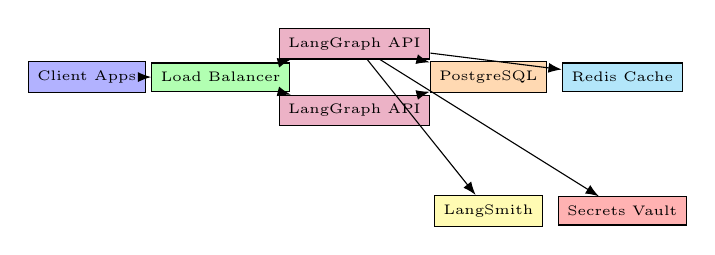
\begin{tikzpicture}[scale=0.85, every node/.style={font=\tiny}]
\node[draw,rectangle,fill=blue!30] (client) at (0,3) {Client Apps};
\node[draw,rectangle,fill=green!30] (lb) at (2,3) {Load Balancer};
\node[draw,rectangle,fill=purple!30] (api) at (4,3.5) {LangGraph API};
\node[draw,rectangle,fill=purple!30] (api2) at (4,2.5) {LangGraph API};
\node[draw,rectangle,fill=orange!30] (db) at (6,3) {PostgreSQL};
\node[draw,rectangle,fill=cyan!30] (cache) at (8,3) {Redis Cache};
\node[draw,rectangle,fill=yellow!30] (smith) at (6,1) {LangSmith};
\node[draw,rectangle,fill=red!30] (vault) at (8,1) {Secrets Vault};
\draw[-{Latex}] (client) -- (lb);
\draw[-{Latex}] (lb) -- (api);
\draw[-{Latex}] (lb) -- (api2);
\draw[-{Latex}] (api) -- (db);
\draw[-{Latex}] (api2) -- (db);
\draw[-{Latex}] (api) -- (cache);
\draw[-{Latex}] (api) -- (smith);
\draw[-{Latex}] (api) -- (vault);
\end{tikzpicture}
\end{center}
\docref{Production Infrastructure}
\end{frame}

\begin{frame}{Cost Management Strategies}
\setlength{\itemsep}{1pt}
\begin{itemize}
\item \textbf{Model selection:} GPT-4 vs. GPT-3.5; weigh cost vs. quality
\item \textbf{Caching:} Reuse embeddings, tool results, API responses
\item \textbf{Batch processing:} Process multiple queries at once if latency allows
\item \textbf{Budget alerts:} Monitor token spend; alert on spikes
\item \textbf{Reserved capacity:} Negotiate volume discounts with API providers
\end{itemize}
\vspace{0.15cm}
\begin{tipbox}[ROI Focus]
If agent saves 1 hour/week × \$100/hour, can afford \$10/day in API costs.
\end{tipbox}
\end{frame}

\begin{frame}{Common Production Pitfalls}
\setlength{\itemsep}{1pt}
\begin{itemize}
\item \textbf{No monitoring:} Errors happen silently; no visibility into failures
\item \textbf{No rate limiting:} Malicious user triggers runaway costs
\item \textbf{Untested graphs:} Works on laptop; fails in production at scale
\item \textbf{Hardcoded secrets:} API keys exposed in source control
\item \textbf{No error handling:} Single node failure crashes entire system
\item \textbf{Token bleed:} Messages accumulate forever; token cost explodes
\end{itemize}
\vspace{0.1cm}
\docref{Production Lessons Learned}
\end{frame}

\begin{frame}{Summary: Deploying to Production}
\setlength{\itemsep}{1pt}
\begin{enumerate}
\item Choose deployment mode: Cloud (managed) or self-hosted (control)
\item Configure \texttt{langgraph.json} with graph definition, dependencies
\item Write comprehensive unit and integration tests
\item Enable LangSmith tracing and monitoring
\item Implement input validation and secrets management
\item Set up token budgets, rate limiting, error handlers
\item Deploy with \texttt{langgraph deploy}; monitor from day 1
\item Optimize for latency and cost based on metrics
\end{enumerate}
\vspace{0.15cm}
\docref{Deployment Checklist}
\end{frame}

\begin{frame}{Cheat Sheet: Production Essentials}
\small
\begin{tabular}{ll}
\toprule
\textbf{Concern} & \textbf{Solution} \\
\midrule
Hosting & LangGraph Cloud (managed) \\
Persistence & PostgreSQL checkpointing \\
Monitoring & LangSmith tracing + dashboards \\
Scaling & Auto-scaling (Cloud) or Kubernetes (self-hosted) \\
Security & API keys, OAuth, input validation \\
Cost control & Token budgets, caching, model selection \\
Observability & Structured logging, traces, alerts \\
Testing & Unit, integration, load tests \\
\bottomrule
\end{tabular}
\end{frame}

\begin{frame}{Self-Check Questions}
\setlength{\itemsep}{2pt}
\begin{enumerate}
\item What's the difference between LangGraph Cloud and self-hosted?
\item How would you prevent prompt injection in user queries?
\item What metrics would you monitor in LangSmith?
\item How would you implement a token budget for cost control?
\item What's a canary deployment, and why is it safer?
\item How would you handle a sudden spike in API costs?
\item What should be in your langgraph.json file?
\end{enumerate}
\end{frame}

\end{document}
